\documentclass[a4paper,11pt]{article}

% ── Packages ──────────────────────────────────────────────────────────────────
\usepackage[
  a4paper,
  top=0.6cm,
  bottom=0.6cm,
  left=0.8cm,
  right=0.8cm
]{geometry}

\usepackage[T1]{fontenc}
\usepackage[utf8]{inputenc}
\usepackage[sfdefault]{inter}
\usepackage{textcase}
\usepackage{graphicx}
\usepackage{tikz}
\usepackage{fontawesome5}
\usepackage{array}
\usepackage{tabularx}
\usepackage{titlesec}
\usepackage{xcolor}
\usepackage{microtype}
\usepackage{hyperref}
\usepackage{enumitem}

\pagestyle{empty}
\setlength{\parindent}{0pt}

% ── Color Palette ─────────────────────────────────────────────────────────────
\definecolor{primaryblue}{RGB}{0, 75, 160}      % Deep professional blue
\definecolor{accentblue}{RGB}{0, 130, 220}     % Brighter blue for links/accents
\definecolor{darkgray}{RGB}{35, 35, 35}        % Primary body text
\definecolor{subtext}{RGB}{85, 85, 85}          % Metadata / Subtitles
\definecolor{rulecolor}{RGB}{200, 210, 225}     % Section dividers
\definecolor{lightbg}{RGB}{245, 247, 250}       % Photo background box

% ── Hyperlink Styling ────────────────────────────────────────────────────────
\hypersetup{
  colorlinks=true,
  urlcolor=accentblue,
  linkcolor=accentblue
}

% ── Section Styling ──────────────────────────────────────────────────────────
\titleformat{\section}
  {\Large\bfseries\color{primaryblue}}
  {}{0em}{\MakeTextUppercase}
  [\vspace{-10pt}{\color{primaryblue}\rule{\linewidth}{0.4pt}}\vspace{-2pt}]
\titlespacing*{\section}{0pt}{2pt}{-1pt}

% ── Table Alignment Helpers ──────────────────────────────────────────────────
\newcolumntype{L}{>{\raggedright\arraybackslash}p{2.3cm}}
\newcolumntype{G}{>{\raggedleft\arraybackslash}p{2.6cm}}
\renewcommand{\arraystretch}{1.08}

\newcommand{\role}[1]{{\itshape\color{subtext} #1}}
\newcommand{\meta}[1]{{\itshape\color{subtext} #1}}

% ── Document Start ───────────────────────────────────────────────────────────
\begin{document}
\color{darkgray}

% ── Header ────────────────────────────────────────────────────────────────────
\noindent
\begin{minipage}[c]{0.74\linewidth}
  {\fontsize{26}{30}\selectfont \textbf{\color{primaryblue}Kartavya Suryawanshi}}\\[5pt]
  \normalsize
  \faMapMarker*\ IIT Mandi, Kamand, Himachal Pradesh, India\\[3pt]
  \faPhone\ +91 86689 44955
  \quad\textbullet\quad
  \faEnvelope\ \href{mailto:b24199@students.iitmandi.ac.in}{b24199@students.iitmandi.ac.in}\\[3pt]
  \faLinkedin\ \href{https://www.linkedin.com/in/kartavya-suryawanshi-918753320/}{LinkedIn}
  \quad\textbullet\quad
  \faGithub\ \href{https://github.com/Kartavya728}{GitHub}\\[3pt]
  \textbf{Date of Birth:} 28.07.2006
  \quad\textbullet\quad
  \textbf{Place of Birth:} Pune, India
\end{minipage}%
\hfill
\begin{minipage}[c]{0.23\linewidth}
  \centering
  \begin{tikzpicture}
    % Shadow/Back Box
    \node[
      fill=primaryblue!15,
      minimum width=2.7cm,
      minimum height=2.7cm,
      rounded corners=4pt
    ] at (0.08,-0.08) {};
    % Main Frame Box
    \node[
      fill=lightbg,
      rounded corners=4pt,
      draw=primaryblue,
      line width=1.1pt,
      inner sep=1.5pt
    ] at (0,0) {
      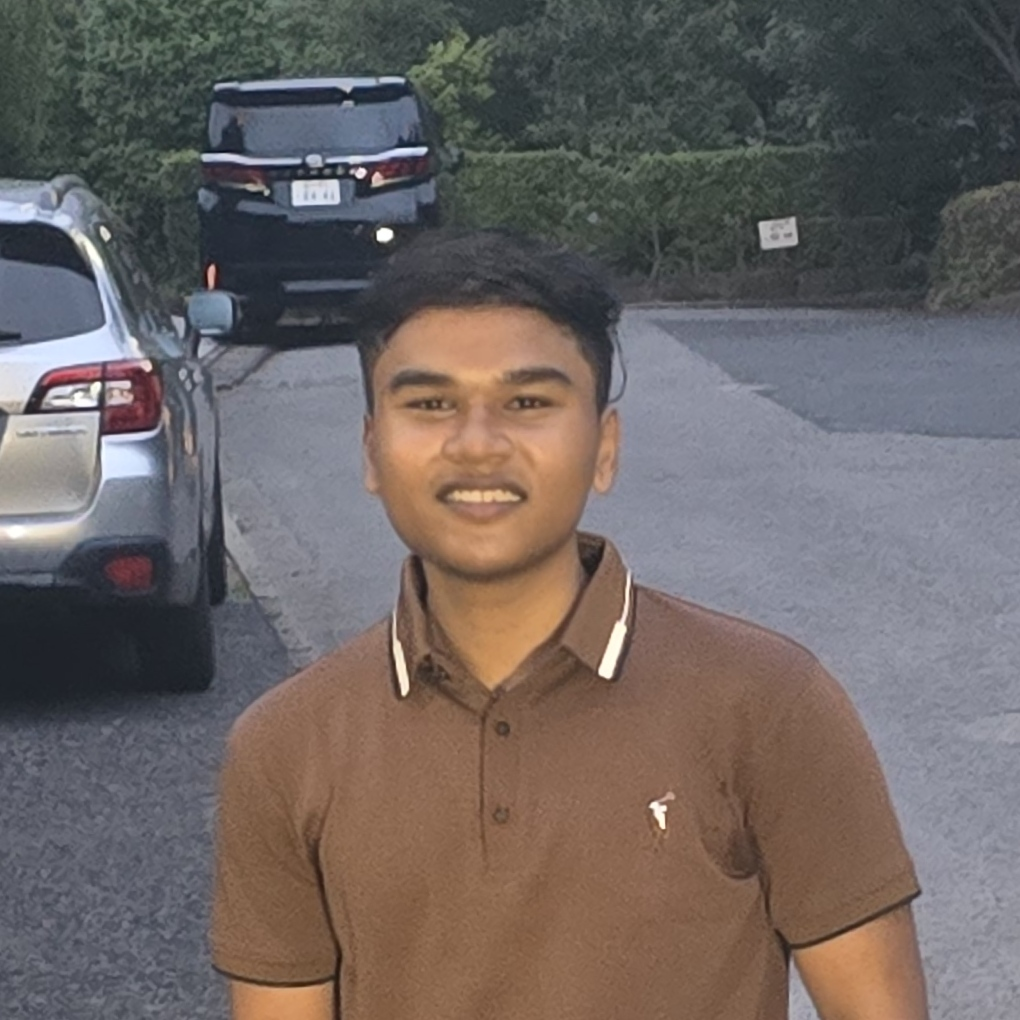
\includegraphics[width=2.6cm,height=2.6cm,keepaspectratio]{pro.jpeg}
    };
  \end{tikzpicture}
\end{minipage}

\vspace{4pt}
% Two-tone colored bar under header
\noindent
{\color{primaryblue}\rule{0.7\linewidth}{1.8pt}}{\color{accentblue}\rule{0.3\linewidth}{1.8pt}}
\vspace{-1pt}

% ── About Me ──────────────────────────────────────────────────────────────────
\section*{About Me}
\normalsize
Driven Data Science undergraduate at IIT Mandi (\textbf{CGPA 9.27/10}) with strong expertise in machine learning, deep learning, and full-stack software development. Proven track record of turning complex technical concepts into real-world applications across enterprise analytics and web engineering internships, alongside four national-level hackathon victories. Passionate about architecting scalable AI models and high-performance data systems.

% ── Higher Education ──────────────────────────────────────────────────────────
\section*{Higher Education}
\begin{tabularx}{\linewidth}{L X G}
2024 -- present & \textbf{Indian Institute of Technology Mandi (IIT Mandi)}, India\newline
\role{B.Tech.\ in Data Science \& Engineering (DSE)} & \textbf{\color{primaryblue}CGPA: 9.27 / 10} \\[3pt]
& \multicolumn{2}{p{15.4cm}}{\normalsize\textbf{Relevant Coursework:} Data Structures \& Algorithms, Machine Learning, Deep Learning, Matrix Computations, Systems for Data Processing, Linear Algebra, Computer Organization}
\end{tabularx}

% ── School Education ──────────────────────────────────────────────────────────
\section*{School Education}
\begin{tabularx}{\linewidth}{L X G}
2021 -- 2023 & \textbf{Jadhavar Jr.\ College}, Pune, Maharashtra, India\newline
\role{Higher Secondary Certificate (Class XII) --- HSC Board} & \textbf{86.0\%} \\[3pt]
2016 -- 2021 & \textbf{NAJ Academy High School}, Murud Janjira, Maharashtra, India\newline
\role{Secondary School Certificate (Class X) --- SSC Board} & \textbf{91.4\%}
\end{tabularx}

% ── Professional Experience ───────────────────────────────────────────────────
\section*{Professional Experience}

\begin{tabularx}{\linewidth}{L X G}
06/2026 -- 07/2026 &
\textbf{Nomura Real Estate Holdings}, Tokyo, Japan \newline
\role{Data Analytics Intern} & \\[-11pt]

& \multicolumn{2}{p{15.4cm}}{\normalsize
\begin{itemize}[leftmargin=1.1em, topsep=0pt, itemsep=0pt, parsep=0pt]
    \item Built automated \textbf{Power BI} dashboards using \textbf{Microsoft Viva Insights} to analyze enterprise productivity data.
    \item Identified workflow bottlenecks through statistical analysis, supporting data-driven decisions.
\end{itemize}} \\[1pt]

08/2025 -- 12/2025 &
\textbf{Finance Department, IIT Mandi}, Himachal Pradesh, India \newline
\role{Full-Stack Developer Intern} & \\[-11pt]

& \multicolumn{2}{p{15.4cm}}{\normalsize
\begin{itemize}[leftmargin=1.1em, topsep=0pt, itemsep=0pt, parsep=0pt]
    \item Developed a fund management portal using \textbf{React.js}, \textbf{Node.js}, and \textbf{PostgreSQL}.
    \item Implemented grant tracking and RBAC to streamline financial operations.
\end{itemize}}
\end{tabularx}

% ── Achievements ──────────────────────────────────────────────────────────────
\section*{Achievements}
\begin{tabularx}{\linewidth}{L X}
2025 & \textbf{Winner} --- \href{https://www.spaceappschallenge.org/}{NASA Space Apps Challenge} (1st/100+ teams): Built \textit{Astrogenesis}, a RAG-powered bioscience research engine. \\[2.5pt]
2025 & \textbf{Winner} --- \href{https://www.ihub-data.iiit.ac.in/}{iHub Multimodal AI Hackathon} (1st/1,600+ teams): Led end-to-end development of \textit{Smarts Scribe}, an AI lecture assistant. \\[2.5pt]
2026 & \textbf{Winner} --- \href{https://www.hcltech.com/}{Hack 60 (HCLTech $\times$ IIT Mandi)}: 1st place in Deep-Learning track for a real-time deepfake \& audio anti-spoofing system. \\[2.5pt]
2026 & \textbf{1st Runner-Up} --- \href{https://frosthack.com/}{Frosthack IIT Mandi} (2nd/50+ teams): Built autonomous multi-agent AI task orchestration pipelines.
\end{tabularx}


% ── Skills ────────────────────────────────────────────────────────────────────

\section*{Skills}

\renewcommand{\arraystretch}{0.8}
\setlength{\tabcolsep}{3pt}

% Shift only the content cells down by 0.1cm
\newcommand{\skillcell}[1]{\raisebox{-0.2cm}{#1}}

\begin{center}
\begin{tabularx}{\linewidth}{|>{\bfseries\color{primaryblue}}p{2.2cm}|X|}
\hline

Languages &
\skillcell{C, C++, Python, JavaScript, TypeScript, HTML, CSS, SQL} \\ \hline

Frameworks &
\skillcell{React.js, Next.js, Node.js, Express.js, Django, FastAPI, Tailwind CSS, LangChain, Streamlit} \\ \hline

ML/DL &
\skillcell{PyTorch, TensorFlow, Scikit-learn, CNNs, Transformers, Autoencoders, LLMs, RAG} \\ \hline

Tools &
\skillcell{Git, Docker, Kubernetes, PostgreSQL, Supabase, Redis, MongoDB, AWS, Railway} \\ \hline

Spoken &
\skillcell{English (C1), Hindi, Marathi (Native)} \\ \hline

\end{tabularx}
\end{center}

\vspace{0.2cm}

\end{document}